\documentclass{beamer}
\usepackage{ctex}
\usepackage{minted}
\usepackage{smartdiagram}
\usetikzlibrary{positioning}
\usetheme{metropolis}           % Use metropolis theme
\title{Flink Window API}
\date{\today}
\author{左元}
\institute{尚硅谷 大数据组}
\begin{document}
  \maketitle
  \begin{frame}
    \frametitle{主要内容}

    \begin{itemize}
        \item Window概念
        \item Window类型
        \item Window API
    \end{itemize}
  
  \end{frame}

  \begin{frame}
      \frametitle{窗口(Window)}

      \begin{figure}
        \centering
        \includegraphics[width=0.8\textwidth]{image25.png}
        \caption{无界流}
      \end{figure}
  
      \begin{itemize}
          \item 一般真实的流都是无界的,怎样处理无界的数据?
          \item 可以把无限的数据流进行切分,得到有限的数据集进行处理 —— 也就是得到有界流
          \item 窗口(Window)就是将无限流切割为有限流的一种方式,它会将流数据分发到有限大小的桶(bucket)中进行分析
      \end{itemize}
  
  \end{frame}

  \begin{frame}
      \frametitle{Window类型}
  
      \begin{itemize}
          \item 时间窗口(Time Window)
          \begin{itemize}
              \item 滚动时间窗口
              \item 滑动时间窗口
              \item 会话窗口(只有Flink支持)
          \end{itemize}
          \item 计数窗口(Count Window)
          \begin{itemize}
              \item 滚动计数窗口
              \item 滑动计数窗口
          \end{itemize}
      \end{itemize}
  
  \end{frame}

  \begin{frame}
      \frametitle{滚动窗口(Tumbling Windows)}

      \begin{figure}
        \centering
        \includegraphics[width=0.6\textwidth]{tumbling-windows.pdf}
        \caption{滚动窗口}
      \end{figure}
  
      \begin{itemize}
          \item 将数据依据固定的窗口长度对数据进行切分
          \item 时间对齐,窗口长度固定,没有重叠
      \end{itemize}
  
  \end{frame}

  \begin{frame}
      \frametitle{滑动窗口(Sliding Windows)}

      \begin{figure}
        \centering
        \includegraphics[width=0.6\textwidth]{sliding-windows.pdf}
        \caption{滑动窗口}
      \end{figure}
  
      \begin{itemize}
          \item 滑动窗口是固定窗口的更广义的一种形式,滑动窗口由固定的窗口长度和滑动间隔组成
          \item 窗口长度固定,可以有重叠
      \end{itemize}
  
  \end{frame}

  \begin{frame}
      \frametitle{会话窗口(Session Windows)}

      \begin{figure}
        \centering
        \includegraphics[width=0.6\textwidth]{session-windows.pdf}
        \caption{会话窗口}
      \end{figure}
  
      \begin{itemize}
          \item 由一系列事件组合一个指定时间长度的 timeout 间隙组成,也就是一段时间没有接收到新数据就会生成新的窗口
          \item 特点:时间无对齐
          \item 只有Flink支持会话窗口
      \end{itemize}
  
  \end{frame}

  \begin{frame}
      \frametitle{Window API}
  
      \begin{itemize}
          \item 窗口分配器 —— window() 方法
          \item 我们可以用.window()来定义一个窗口,然后基于这个window去做一些聚合或者其它处理操作。
      \end{itemize}
  
  \end{frame}

  \begin{frame}
      \frametitle{创建不同类型的窗口}
  
      \begin{itemize}
          \item 处理时间窗口
          \item 事件时间窗口
      \end{itemize}
  
  \end{frame}

  \begin{frame}[fragile]
      \frametitle{处理时间窗口}
  
      \begin{itemize}
          \item 滚动窗口
            \begin{minted}[breaklines,fontsize=\footnotesize]{java}
.window(TumblingProcessingTimeWindows.of(Time.seconds(5)))
            \end{minted}
          \item 滑动窗口
            \begin{minted}[breaklines,fontsize=\footnotesize]{java}
.window(SlidingProcessingTimeWindows.of(Time.seconds(10), Time.seconds(5)))
            \end{minted}
          \item 会话窗口
            \begin{minted}[breaklines,fontsize=\footnotesize]{java}
.window(ProcessingTimeSessionWindows.withGap(Time.seconds(10)))
            \end{minted}
      \end{itemize}
  
  \end{frame}

  \begin{frame}[fragile]
      \frametitle{事件时间窗口}
  
      \begin{itemize}
          \item 滚动窗口
            \begin{minted}[breaklines,fontsize=\footnotesize]{java}
.window(TumblingEventTimeWindows.of(Time.seconds(5)))
            \end{minted}
          \item 滑动窗口
            \begin{minted}[breaklines,fontsize=\footnotesize]{java}
.window(SlidingEventTimeWindows.of(Time.seconds(10), Time.seconds(5)))
            \end{minted}
          \item 会话窗口
            \begin{minted}[breaklines,fontsize=\footnotesize]{java}
.window(EventTimeSessionWindows.withGap(Time.seconds(10)))
            \end{minted}
      \end{itemize}
  
  \end{frame}

  \begin{frame}
      \frametitle{窗口聚合函数}
  
      \begin{itemize}
          \item 窗口聚合函数定义了要对窗口中收集的数据做的计算操作
          \item 可以分为两类
          \begin{itemize}
              \item 增量聚合函数
              \item 全窗口聚合函数
          \end{itemize}
      \end{itemize}
  
  \end{frame}

  \begin{frame}
      \frametitle{增量聚合函数}
  
      \begin{itemize}
          \item 每条数据到来就进行计算,只保存一个简单的状态(累加器)
          \item ReduceFunction, AggregateFunction
          \item 当窗口闭合的时候,增量聚合完成
          \item 处理时间:当机器时间超过窗口结束时间的时候,窗口闭合
          \item 来一条数据计算一次
      \end{itemize}
  
  \end{frame}

  \begin{frame}
      \frametitle{增量聚合函数}
  
      \begin{figure}
        \centering
        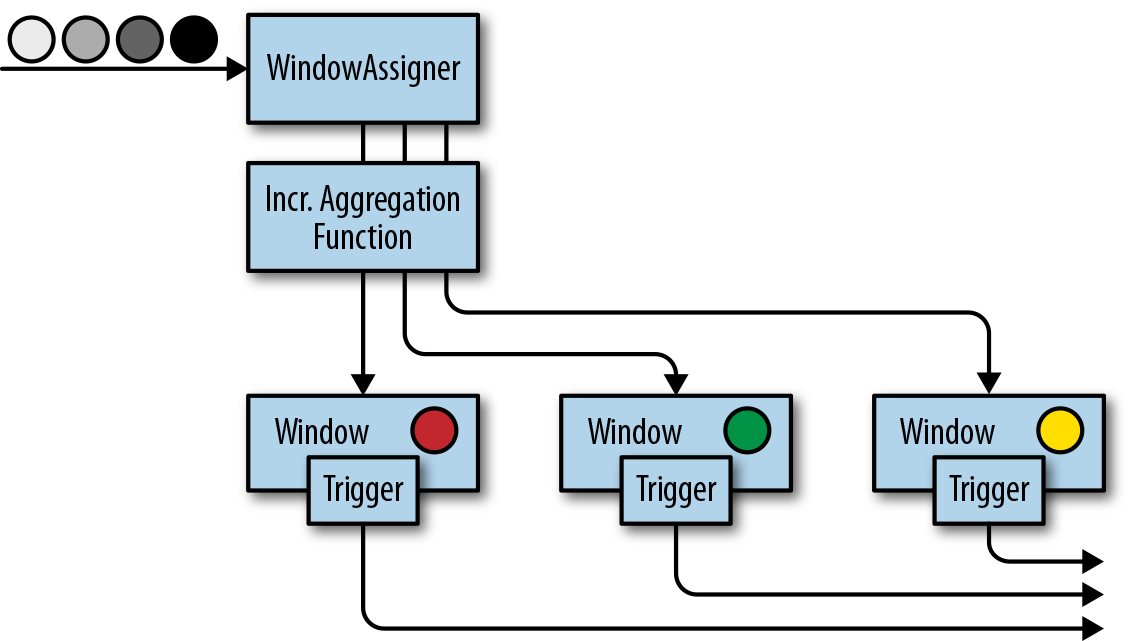
\includegraphics[width=0.6\textwidth]{spaf_0604.png}
        \caption{增量聚合函数}
      \end{figure}
  
  \end{frame}

  \begin{frame}
      \frametitle{全窗口聚合函数}
  
      \begin{itemize}
          \item 先把窗口所有数据收集起来,等到计算的时候会遍历所有数据
          \item ProcessWindowFunction
      \end{itemize}
  
  \end{frame}

  \begin{frame}
      \frametitle{全窗口聚合函数}
  
      \begin{figure}
        \centering
        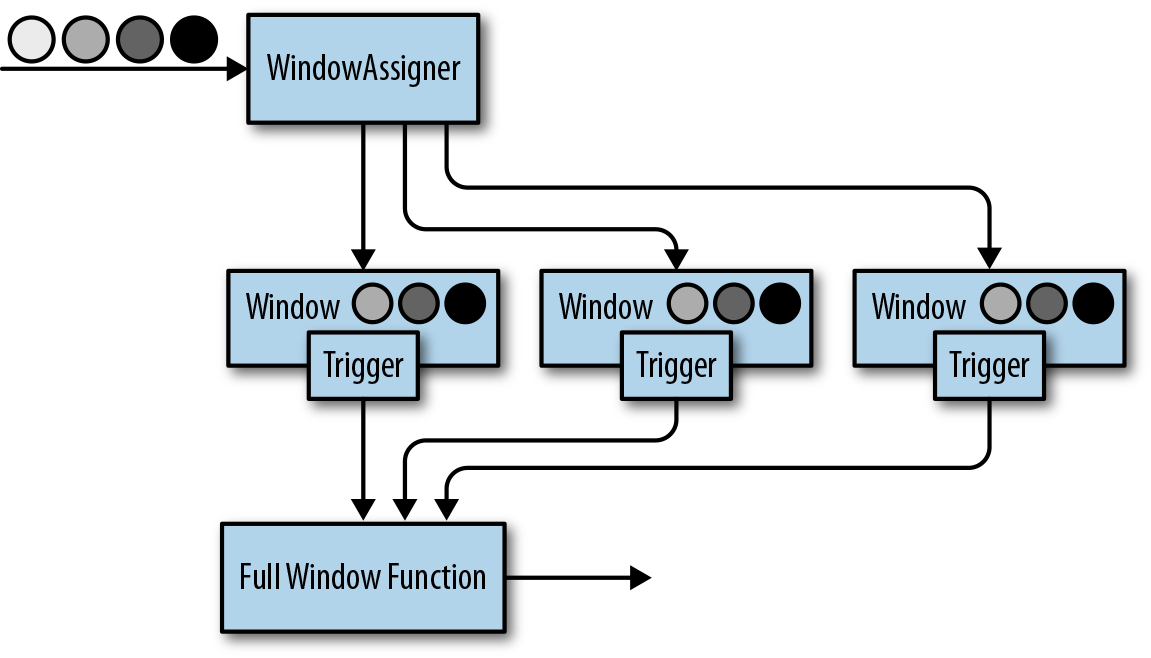
\includegraphics[width=0.6\textwidth]{spaf_0605.png}
        \caption{全窗口聚合函数}
      \end{figure}
  
  \end{frame}

  \begin{frame}
      \frametitle{增量聚合和全窗口聚合结合使用}
  
      \begin{itemize}
          \item 可以访问窗口信息
          \item 不需要收集窗口中的所有元素,只需要维护一个累加器,节省内存
      \end{itemize}
  
  \end{frame}

  \begin{frame}
      \frametitle{增量聚合和全窗口聚合结合使用}
  
      \begin{figure}
        \centering
        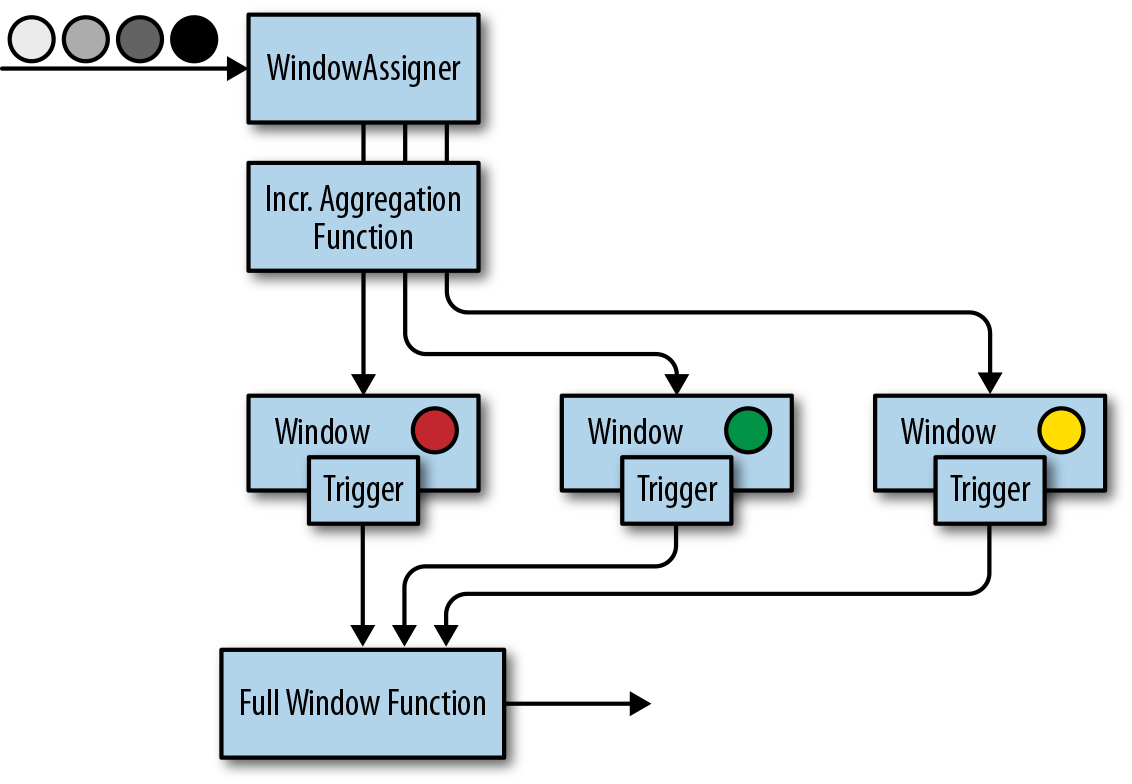
\includegraphics[width=0.6\textwidth]{spaf_0606.png}
        \caption{增量聚合和全窗口聚合结合使用}
      \end{figure}
  
  \end{frame}

  \begin{frame}
      \frametitle{其他可选API}
  
      \begin{itemize}
          \item .trigger() —— 触发器
          \begin{itemize}
              \item 定义窗口什么时候关闭,触发计算并输出结果
          \end{itemize}
          \item .evictor() —— 移除器
          \begin{itemize}
              \item 定义移除某些数据的逻辑
          \end{itemize}
          \item .allowedLateness() —— 允许处理迟到的数据
          \item .sideOutputLateData() —— 将迟到的数据放入侧输出流
          \item .getSideOutput() —— 获取侧输出流
      \end{itemize}
  
  \end{frame}

  \begin{frame}[fragile]
      \frametitle{基于Key的窗口}
  
\begin{minted}[breaklines,fontsize=\tiny]{java}
stream
    .keyBy(...)               <-  keyed versus non-keyed windows
    .window(...)              <-  required: "assigner"
    [.trigger(...)]            <-  optional: "trigger" (else default trigger)
    [.evictor(...)]            <-  optional: "evictor" (else no evictor)
    [.allowedLateness(...)]    <-  optional: "lateness" (else zero)
    [.sideOutputLateData(...)] <-  optional: "output tag" (else no side output for late data)
    .reduce/aggregate/fold/apply()      <-  required: "function"
    [.getSideOutput(...)]      <-  optional: "output tag"
\end{minted}
  
  \end{frame}

  \begin{frame}[fragile]
      \frametitle{不分流直接开窗口}
  
\begin{minted}[breaklines,fontsize=\tiny]{java}
stream
    .windowAll(...)           <-  required: "assigner"
    [.trigger(...)]            <-  optional: "trigger" (else default trigger)
    [.evictor(...)]            <-  optional: "evictor" (else no evictor)
    [.allowedLateness(...)]    <-  optional: "lateness" (else zero)
    [.sideOutputLateData(...)] <-  optional: "output tag" (else no side output for late data)
    .reduce/aggregate/fold/apply()      <-  required: "function"
    [.getSideOutput(...)]      <-  optional: "output tag"
\end{minted}
  
  \end{frame}

  \begin{frame}[plain,c]
    %\frametitle{A first slide}
    
    \begin{center}
    \Huge Q \& A
    \end{center}
    
  \end{frame}

\end{document}